\begin{frame}{Restricciones}
  Restricciones:
  \begin{itemize}[<+->]
  \item La función de transición suave MIX sólo funciona en objetos
    geométricos $f$-fat con $f \in \mathbb{R}$ y $f>0$.
    \begin{figure}  
      \centering
      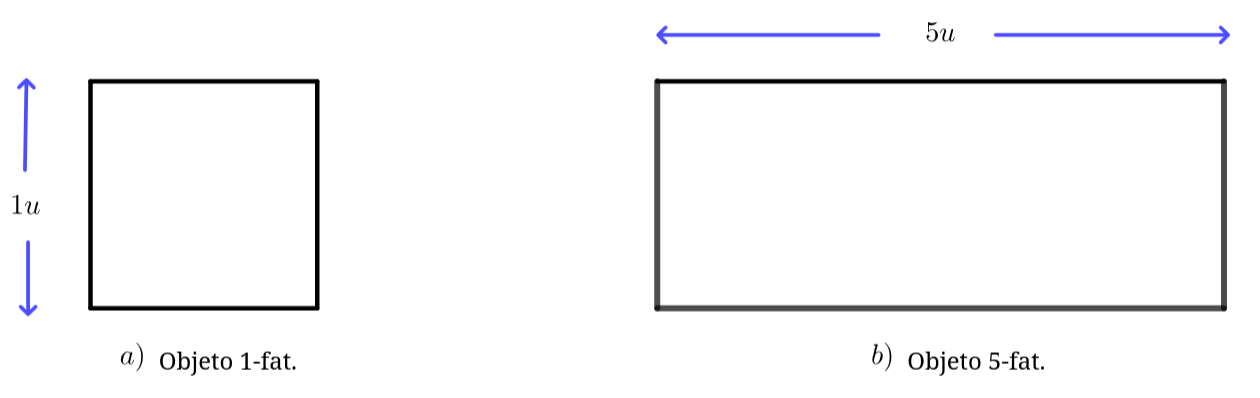
\includegraphics[width=0.7\textwidth]{./Images/fat.png}
    \end{figure}
  \item La función recibe dos estados $S_i, S_f$ y transita de $S_i$
    a $S_f$ en $\mathcal{O}(\alpha \log \alpha)$, pues debe ordenar
    cada conjunto de entrada.
  \item Sólo funciona para $\mathbb{R}^d$ con $d$ constante.
  \item Se pueden realizar, a lo más, $5u$ eliminaciones o adiciones,
    con $u \in \mathbb{Z}^+$, asumiendo $u > 0$.
  \item Las eliminaciones se realizan de manera directa, las adiciones
    se realizan al final de la ejecución del algoritmo. Basta guardar
    las adiciones en una cola.
  \item La cantidad de conjuntos candidatos es $K \in \mathcal{O}(1)$.
  \end{itemize}
\end{frame}
